\chapter{Key-value model, MapReduce and Hadoop} % (fold)
\label{cha:background}

This chapter introduces some concepts that are used in the subsequent sections:
the key-value model, MapReduce paradigm and Hadoop framework.

\section{Key-value model}\label{section:mapreduce}

Key-value model is a simplified model for data storage. It is based on one linked
pair: the key and the value. Generally the pair is stored pure without aggregation or
any creation of data schema, thus all detailing of data is done in runtime. Unlike
other models such as relational model~\cite{codd:1970} in which the simplistic notion
of relation already gives some sense for the data, similarly to the hierarchical
data model~\cite{silber:2005} in which the links that connect the records give
details for the data.

To solve some particularities involving relational model was created data warehouse,
it is a repository that aggregates data from several sources ~\cite{silber:2005},
to make such aggregations is used the technique Extract Transform Load(\textbf{ETL}),
the data are extracted from sources, so they are transformed and load in a data
warehouse.

Due the simple storage of the data in key-value model the data \textit{transformation}
is done in the last fase, in other words, the data make sense when they are required,
there is a inversion of ETL to ELT(Extract Load Transform), but such inversion
cause one trouble to process a large amount of data, thus one big computing
power is necessary to query the data. One programming paradigm that handles the
key-value model is the MapReduce, it is going to present in the next section.

\section{MapReduce}\label{section:mapreduce}
MapReduce is a programming system for high-level that allow many processes of one
database can be written in simple way, according by Molina~\cite{molina:2009}.
That database processes aim to process a large amount of data that are splitted
and assigned to set computers, called computers cluster. Thus can improve the
performance obtained by parallelism, omitting all complexity for that the user
focus stays in the main problem that is the data processing.

The MapReduce paradigm have been implemented under key-value model, it was created
to process a large amount of data and benefits from data parallelism, consequently
builds large-scale parallel data processing applications. The paradigm is inspired
on the high-level \textbf{Map} and \textbf{Reduce} primitives from functional
programming languages. Hence the programmers can focus only in creation of the two
higher-order funcions to solve a specific problem and to generate the necessary
data, so it can just define the precice behavior of those functions.

Acording by\cite{dean:2008}: "the computation takes a set of \textit{input}
key/value pairs, and produces a set of \textit{output} key/value pairs.". The user
write the map function that receives a set of input key/value pair and produces an
\textit{intermidiate} set of key/value pairs. The reduce function written for the
user receives the intermidiate set as input and produces the \textit{resultant}
set of key/value pairs. This process is shown in Figure~\ref{fig:mapReduce}:

\begin{figure}[htbp]
	\centering
	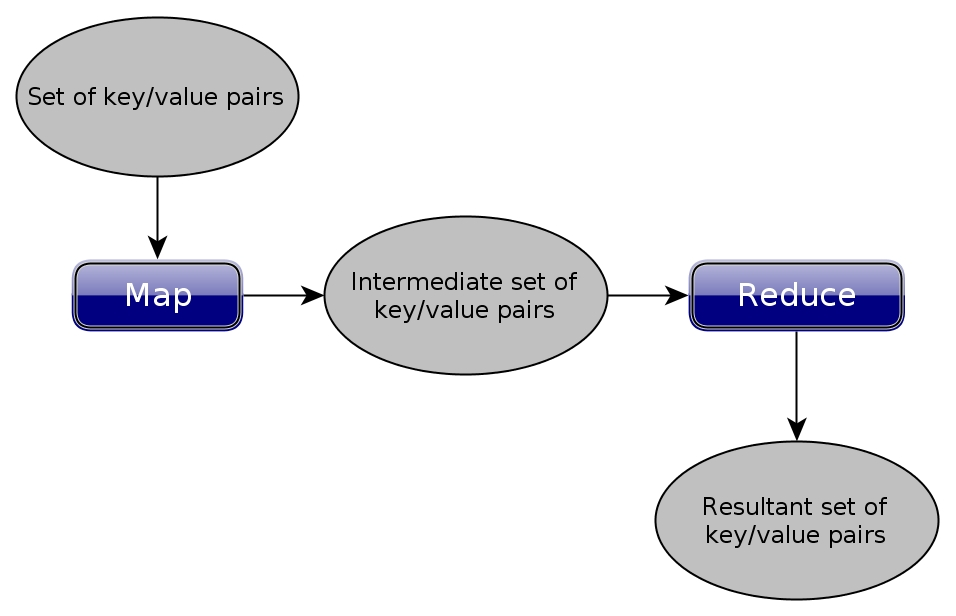
\includegraphics[width=\columnwidth]{img/mapReduce.jpg}
	\caption{Map and Reduce process.}\label{fig:mapReduce}
\end{figure}

\section{Hadoop}
Map and reduce functions are present in Lisp and others functional languages. Recently
the MapReduce paradigm have been implemented by several frameworks such as Greenplum
MapReduce~\cite{Greenplum:2008}, Aster Data~\cite{Aster:2011}, Nokia
Disco~\cite{Mundkur:2011}, Microsoft Dryad~\cite{Isard:2007}, among others. One
open-source implemantation is the Hadoop that is a framework for reliable,
scalable, distributed computing~\cite{hadoop}.

The Hadoop provide an interface to implement the map and reduce functions in high-level.
It was projected for the user focus just on the implementation those functions,
without worrying with the issues involving the distributed computing. All aspects
involving the distributed computing and storage are left to the framework such as
split files, replication, fault tolerance, tasks distribuition etc.

There are two main components on Hadoop:
\begin{itemize}
	\item Hadoop Distributed File System(HDFS);
	\item Engine of MapReduce.
\end{itemize}

The HDFS stores all files in blocks, the block size is configurable per file, all
blocks of one file have the same block size except the last block. It is divide
in two components the \textit{NameNode} and \textit{DataNode}. The NameNode is placed
in one master machine, it store all metedatas and manages all DataNodes, any aspect
involving distributed storage is responsible by this component. The DataNode stores
the data, when one DataNode starts it connects to NameNode, then responds to requests
from the NameNode for filesystem operations.

The engine of MapReduce is responsible by the parallel processing, it is constituted
by one master machine and a lot of slave machines, also called workers. The master
designates which slaves will receive map and reduce tasks with its respective input
blocks. The worker who receive a map task is called mapper and the slave who receive
reduce task is called reducer. All aspects involving the distributed computing
management is responsible by the master like mappers failure, reducers failure,
scheduling tasks, shuffling intermediate files etc.

\subsection{Job processing}

A job is a program in high-level languages(java, ruby or python) that implements the
map and reduce functions. The master machine receive job submission with the relative
input directory in the HDFS where are all files to process. This files must be
inserted previously in the HDFS. Then the master requests to the NameNode infomation
about the blocks and file locations, after that it deploys copies of the job across
several workers.

With the blocks information acquired the map task is scheduled to a set of workers
with its respective input blocks, then the mappers process each input blocks, 
generate key/value intermediate pairs and append its in intermediate files, when
the mapper instance terminate it notify the master. The master splited the intermediate
files in blocks and shuffled it to the reducers to process, when all reducers
intances terminate, they append their result to the final output file. The data
flow between mappers and reducers are shown in Figure~\ref{fig:mrexecute}.


%%Fazer uma nova figura demonstrando o que foi escrito acima
\begin{figure}[htbp]
	\centering
	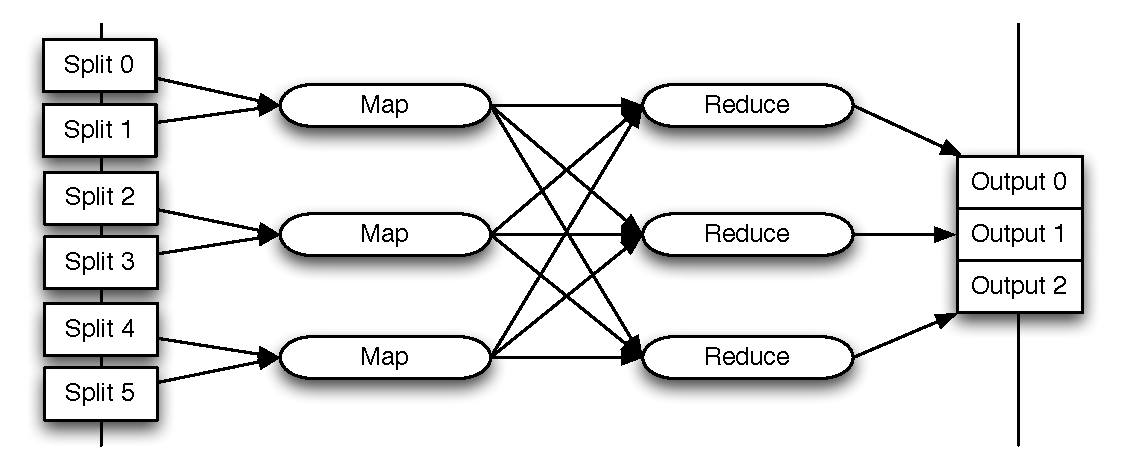
\includegraphics[width=\columnwidth]{img/mapreduce-en.pdf}
%    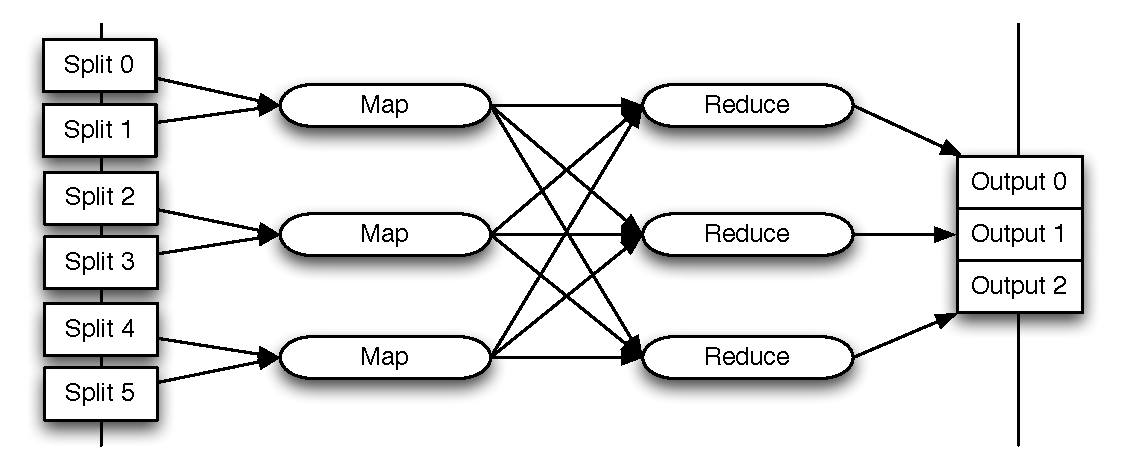
\includegraphics[bb=0 0 1280 960]{img/mapreduce-en.pdf}
	\caption{Execution of Map and Reduce operations}\label{fig:mrexecute}
\end{figure}

The whole processing is based on \tuple{key,value} pairs. The mappers receive the
file blocks, the mappers call the map function and pass the line number as key and
the line as the value, so the pair "line number/line contente" is the \tuple{k1,v1}.
The map generate the intermediate result set of key and values \tuple{set(k2,v2)}, 
when the mappers finished all values for \textit{k2} are agrouped in a list and
the respective pair \tuple{k2, list(v2)} is generated. This pairs are sorted and
pass as input for reducers that generate the result set:

\begin{center}
\begin{tabular}{c c c c}
	\hline
	   map & $k1,v1$ & $\rightarrow$  & $set(k2, v2)$ \\
	   reduce & $k2, list(v2)$ & $\rightarrow$ & $set(v2)$ \\
	\hline
\end{tabular}
\end{center}

Eventually, when the map result are already available in memory, a local reduce
function \emph{Combiner} is used for optimization reasons, then all values for
determinated key are combined, resulting in a local set \tuple{k2, list(v2)}.
This function runs after the Map and before the Reduce functions and is run on
every node that run map functions. The Combiner may be seen as a \emph{mini-reduce}
function, which operates only on data generated by one machine.

A good example of a MapReduce job is the Grep application, which receives as an
input several textual documents and as an output a set of pairs \tuple{Key,Value},
where each key is a different pattern found and the value is the number of occurrences 
of the pattern in the files. The responsibility of the Mapper is to find pattern
in the files and the reduce is to sum the amount found each patterns.

The Java implementation of the map function is presented in Listing~\ref{listing:mapper}. 
The \code{map()} method has four parameters: \code{key}, which is never used; \code{value},
one line that contains the text to be processed; the \code{output}, which will receive
the output pairs and \code{reporter} for debug. The body of the method uses the class
\code{Pattern} to describe a desired pattern, the class \code{Matcher} to find this
pattern, when pattern are found the pair \tuple{matching, 1} is emited to
output.

\singlespacing
\begin{listing}[H]
\begin{minted}[frame=lines,framesep=2mm,fontfamily=courier,fontsize=\scriptsize]{java}
public class RegexMapper<K> extends MapReduceBase
			implements Mapper<K, Text, Text, LongWritable> {

    private Pattern pattern;
    private int group;

    public void configure(JobConf job)
    {
        pattern = Pattern.compile(job.get("mapred.mapper.regex"));
    }

    public void map(K key, Text value, OutputCollector<Text, LongWritable> output,
					Reporter reporter) throws IOException {
        String text = value.toString();
        Matcher matcher = pattern.matcher(text);
        while (matcher.find())
        {
            output.collect(new Text(matcher.group()), new LongWritable(1));
        }
    }
}
\end{minted}
\caption{Class RegexMapper packed in Hadoop~\cite{hadoop}} 
\label{listing:mapper}
\end{listing}

\doublespacing
The implementation of the reduce function is presented in Listing~\ref{listing:reducer}.
The \code{reduce()} method has also four parameters: \code{key}, which contains
a single matching string; \code{values}, a set containing all values associated
to the key (i.e. the matching); \code{output pair}, the resultant pair \tuple{matching,
total} and \code{reporter} for debug. The behavior of the method is quite simple,
it sums all values associated to the key and then writes a pair containing the same
key and the total of matching found.
\singlespacing
\begin{listing}[H]
\begin{minted}[frame=lines,framesep=2mm,fontfamily=courier,fontsize=\scriptsize]{java}
public class LongSumReducer<K> extends MapReduceBase
			 implements Reducer<K, LongWritable, K, LongWritable> {

    public void reduce(K key, Iterator<LongWritable> values,
                     OutputCollector<K, LongWritable> output, Reporter reporter)
                throws IOException {

    // sum all values for this key
    long sum = 0;
    while (values.hasNext())
    {
        sum += values.next().get();
    }

    // output sum
    output.collect(key, new LongWritable(sum));
  }

}
\end{minted}
\caption{Class LongSumReducer packed in Hadoop~\cite{hadoop}} 
\label{listing:reducer}
\end{listing}

\doublespacing
An example of the inputs and the outputs of both functions when applied to a
simple sentence is presented in Table~\ref{table:regexp}. We aplied the following
regular expression: \\ \code{"[a-z]$*$o[a-z]$*$"}, this expression find the words that
contains the vowel \code{o} in the midle of them.

\begin{table}[H]
	\begin{center}
	\begin{tabular}{c p{.4\columnwidth} c p{.3\columnwidth} }
		\hline
		map & "Test for hadoop regular expression inside hadoop" & $\rightarrow$ & \tuple{for,1},\tuple{hadoop,1}, \tuple{expression,1}, \tuple{hadoop,1} \\
		reduce & \tuple{for,\{1\}}, \tuple{hadoop,\{1,1\}}, \tuple{expression,\{1\}} & $\rightarrow$ & \tuple{for,1},\tuple{hadoop,2}, \tuple{expression,1}\\
		\hline
	\end{tabular}
	\end{center}
	\caption{Regular expression example}
	\label{table:regexp}
\end{table}

% chapter chapter_name (end)
